\documentclass[../../../ps_q.tex]{subfiles}

\begin{document}
    \begin{enumerate}
        \item%
            図のように，電気抵抗$\mathrm{R}_1$（抵抗値$R_1$），%
            電気抵抗$\mathrm{R}_2$（抵抗値$R_2$），電気抵抗$\mathrm{R}_3$（抵抗値$R_2$），%
            電気抵抗$\mathrm{R}_4$（抵抗値$R_1$），電気抵抗$\mathrm{R}_5$（抵抗値$r$）%
            からなる回路がある．AB間の合成抵抗$R_\mathrm{T}$を求めよ．\\
            \begin{minipage}{\linewidth}
                \centering
                    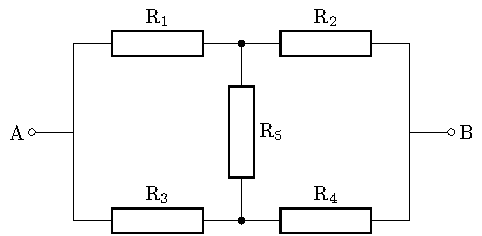
\includegraphics{fig_em_cx_09/fig_em_cx_09_01_q.pdf}
            \end{minipage}
            \vspace{1pt}
        \item%
            図のように，12個の電気抵抗からなる回路がある．いずれの電気抵抗の%
            抵抗値も$R$である．AC間の合成抵抗$R_\mathrm{AC}$を求めよ．\\
            \begin{minipage}{\linewidth}
                \centering
                    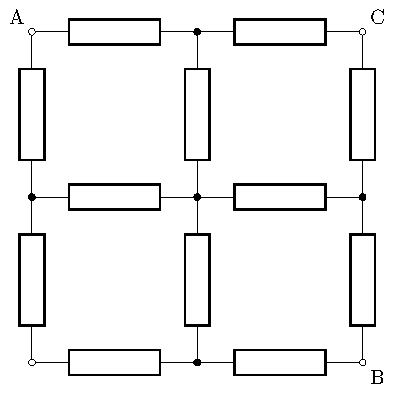
\includegraphics{fig_em_cx_09/fig_em_cx_09_02_q.pdf}
            \end{minipage}
    \end{enumerate}
\end{document}



